%%%%%%%%%%%%%%%%%%%%%%%%% 
%% SITE A GARDER : http://titilog.free.fr/


\documentclass[10pt]{beamer}
% \includeonlyframes{yy}
\usepackage[french]{babel}
\usepackage{color, colortbl}
\definecolor{Gray}{gray}{0.9}
\newcolumntype{g}{>{\columncolor{Gray}}c}
\hypersetup{%
  % pdfborder = {0 0 0},
  colorlinks, urlcolor=blue, linkcolor=, }

\makeatletter \let\@mycite\@cite
\def\@cite#1#2{{\hypersetup{linkcolor=mLightBlue}[{#1\if@tempswa ,
      #2\fi}]}} \makeatother

\usetheme{m} %%%%%
% \usepackage[version=3]{mhchem}
\usepackage{caption}
\captionsetup[figure]{labelformat=empty}
\usepackage{fontspec}
\usepackage{xcolor}
\usepackage{siunitx}
% \usepackage[backend=bibtex]{biblatex} \usepackage[square]{natbib}
% \bibliography{main}
\usepackage[]{algorithm2e}
\usefonttheme[onlymath]{serif} \usepackage{amsmath}
\usepackage{appendixnumberbeamer}
\usepackage{tabularx, booktabs} \usepackage{multirow}
\usepackage{multicol} \usepackage{array} \usepackage{pbox}
\usepackage{mathtools}
\usepackage{adjustbox}
\definecolor{darkred}{HTML}{D38989}
\definecolor{darkgreen}{HTML}{66D191}
\PassOptionsToPackage{enumerate}{shortlabels} \newcommand\ExtraSep
{\dimexpr\cmidrulewidth\relax}
\captionsetup{font=scriptsize,labelfont=scriptsize}
% \addtobeamertemplate{background canvas}{\transfade[duration=0.05]}{}

\usepackage[skip=3pt]{subcaption}
\setlength{\belowcaptionskip}{2pt}
\title{Fusion d'images IRM et MALDI en 3D}
\subtitle{Dernières avancées}

\author{{Florent \textsc{Grélard}\\
    David \textsc{Legland}, Mathieu \textsc{Fanuel}, Loïc \textsc{Foucat}, Hélène \textsc{Rogniaux}}} \titlegraphic{\hspace*{0.18\textwidth}~%
  
\includegraphics[width=0.26\textwidth]{fig/logo-inrae}\hspace*{0.18\textwidth}~%
  
\includegraphics[width=0.26\textwidth]{fig/logo-bibs.png}\hspace*{0.1\textwidth}~%
} \setbeamercolor{bbb}{fg=red}

\let\oldfootnotesize\footnotesize
\renewcommand*{\footnotesize}{\oldfootnotesize\tiny}
\newcommand\labelitemi{$\bullet$}
\renewcommand{\thefootnote}{[\arabic{footnote}]}
% \newrobustcmd*{\footlessfullcite}{\AtNextCite{\renewbibmacro{in:}{}\renewbibmacro{year:}{}}\footfullcite}
% \newrobustcmd*{\lessfullcite}{\AtNextCite{\renewbibmacro{in:}{}\renewbibmacro{year:}{}}\fullcite}

\newcommand{\cfbox}[2]{%
    \colorlet{currentcolor}{.}%
    {\color{#1}%
    \fbox{\color{currentcolor}#2}}%
}


\newcommand{\backupbegin}{ \newcounter{framenumberappendix}
  \setcounter{framenumberappendix}{\value{framenumber}} }
\newcommand{\backupend}{
  \addtocounter{framenumberappendix}{-\value{framenumber}}
  \addtocounter{framenumber}{\value{framenumberappendix}} }
% http://mcclinews.free.fr/latex/introbeamer/les_couleurs.html
\begin{document}

% affiche le logo en bas à droite
% \logo{
\includegraphics[height=0.5cm]{fig/logo-inra}}
% enlève la barre de navigation
\setbeamertemplate{navigation symbols}{ }
\setbeamertemplate{blocks}[rounded][shadow=false]
% Ombre aux blocks
\setbeamertemplate{caption}{\insertcaption}

\date{08 février 2020} % set the Date
% \renewcommand{\insertnavigation}[1]{}

% \AtBeginSection[]{

% }

% \institute{INRAE de Nantes}
\makeatletter
\AtBeginPart{%
  \beamer@tocsectionnumber=0\relax
  \setcounter{section}{0}
}
\makeatother

\begin{frame}[plain]
  \titlepage
\end{frame}


\begin{frame}{Chaîne de traitement 3D : rappels}

  Traitement des images :
  \begin{itemize}
  \item IRM : ajustement de fonctions exponentielles par \textbf{moindres carrés}.
  \item<2-> MALDI : normalisation \textbf{SIC} (Selective Ion Count).
  \end{itemize}

  \visible<2-> {
    \textbf{Calcul :} SIC = TIC - $\sum I_{\text{pics}}$

    \vspace{0.4cm}

    \begin{figure}[ht]
      \centering
      \includegraphics<1>[width=0.7\textwidth]{fig/normalization2}%
      \includegraphics<2>[width=0.7\textwidth]{fig/normalization3}%
      \includegraphics<3>[width=0.7\textwidth]{fig/normalization_sic1}%
      \includegraphics<4>[width=0.7\textwidth]{fig/normalization_sic2}%
      \includegraphics<5>[width=0.7\textwidth]{fig/normalization_sic3}%
      \caption{}
      \label{fig:normalization_sic1}
    \end{figure}
  }
\end{frame}




\begin{frame}{Chaîne de traitement 3D : rappels}
  \begin{itemize}
  \item Détermination des \textbf{correspondances} entre coupes en exploitant les métadonnées.
  \item<2-> Recalage 3D affine utilisant la \textbf{transformée en distance}.
  \end{itemize}

  \visible<2-> {
    \alert{Transformée en distance} : on associe à chaque pixel sa distance au bord de l'objet.

    \begin{figure}[ht]
      \centering
      \begin{subfigure}[t]{0.5\textwidth}
        \centering
        \includegraphics<1>[width=0.65\textwidth]{fig/mri_slice6.png}%
        \includegraphics<2>[width=0.65\textwidth]{fig/mri_slice6_dt.png}
        \caption{}
        \label{subfig:mri_slice6_dt.png}
      \end{subfigure}%
      \begin{subfigure}[t]{0.5\textwidth}
        \centering
        \includegraphics<1>[width=0.65\textwidth]{fig/maldi_slice6.png}%
        \includegraphics<2>[width=0.65\textwidth]{fig/maldi_slice6_dt.png}
        \caption{}
        \label{subfig:maldi_slice6_dt.png}
      \end{subfigure}%
    \end{figure}
  }
\end{frame}

\begin{frame}{Chaîne de traitement 3D : rappels}

  À l'issue du recalage : \textbf{images 3D}.

  Outil de \textbf{visualisation} des images MS 3D.

  \begin{figure}[ht]
    \centering
    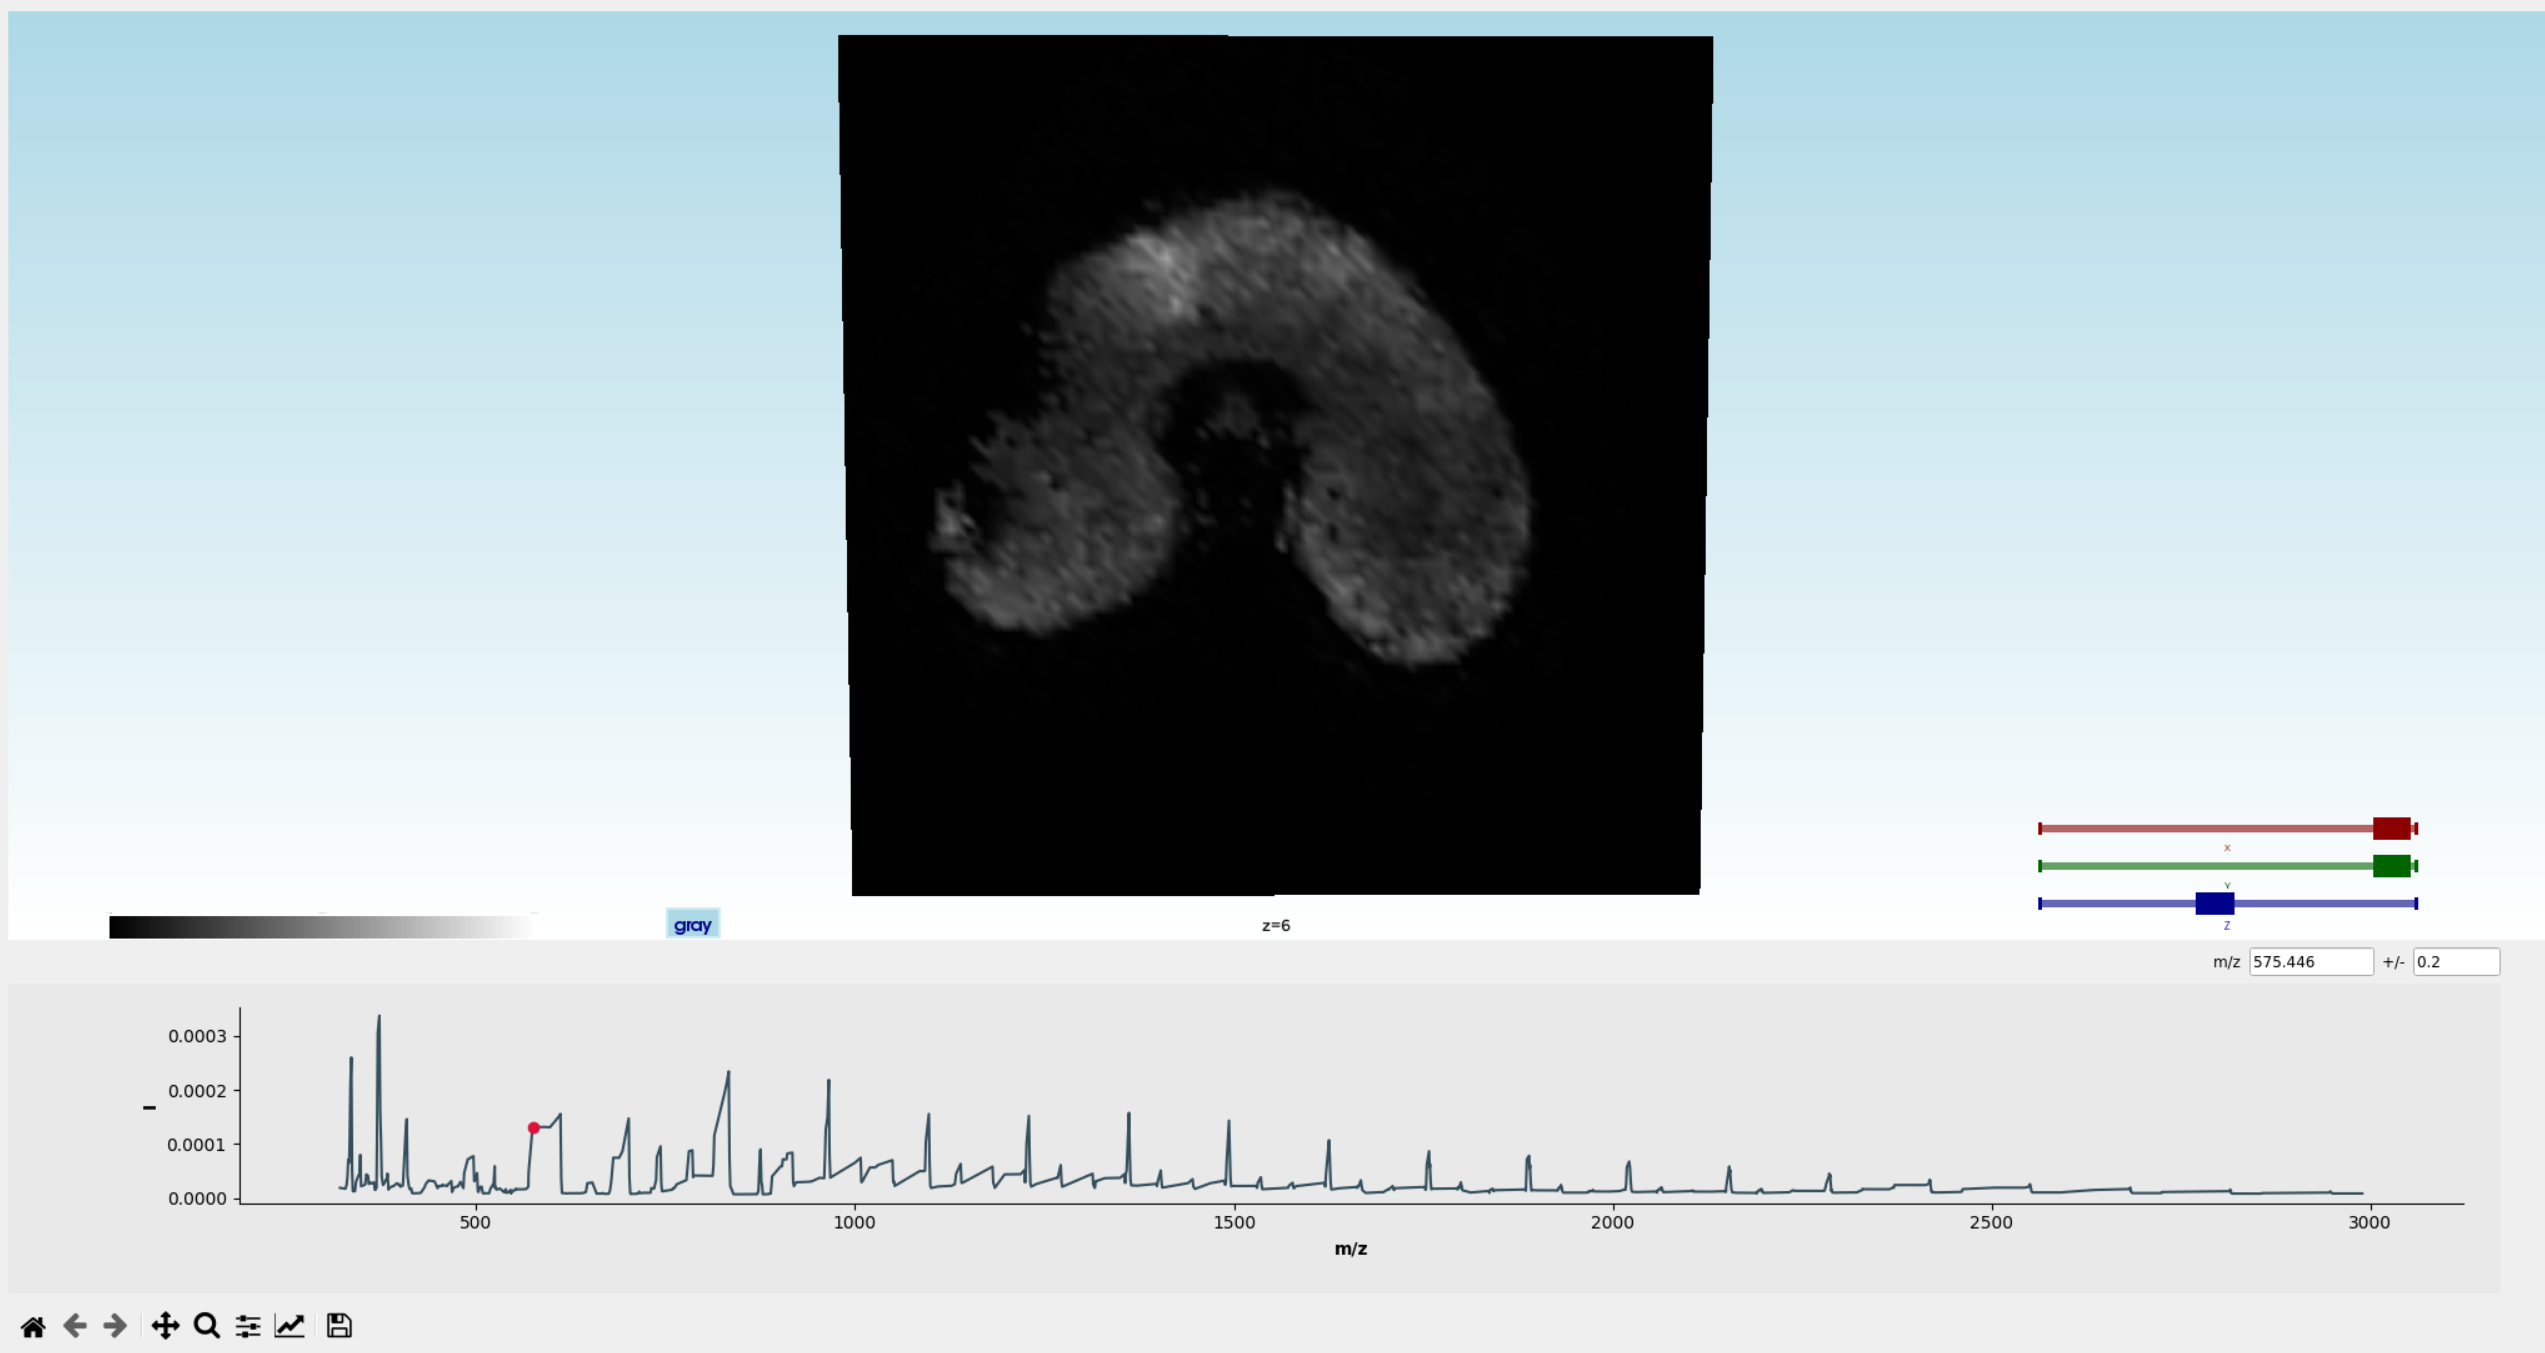
\includegraphics[width=0.95\textwidth]{fig/visu}%
    \caption{}
    \label{fig:visu}
  \end{figure}


\end{frame}


\begin{frame}{Chaîne de traitement 3D : dernières avancées}
  \begin{enumerate}
  \item<2-> Recalage : méthodes \textbf{variationnelles}.
  \item<3-> Analyse statistique : \textbf{nouveaux outils}.
  \end{enumerate}

  \begin{figure}[ht]
    \centering
    \includegraphics<1>[width=0.8\textwidth]{fig/workflow3D_0bis}%
    \includegraphics<2>[width=0.8\textwidth]{fig/workflow3D_5}%
    \includegraphics<3>[width=0.8\textwidth]{fig/workflow3D_6}%
  \end{figure}

  \visible<3-> {
    $\Rightarrow$ Résultats sur variété \textbf{Bobwhite}.
  }
\end{frame}


\AtBeginSection[]{
  \begingroup
  \setbeamercolor{background canvas}{bg=mLightBlue}
  
  \setbeamertemplate{subsection in toc}
  {\leavevmode\leftskip=2em$\bullet$\hskip1em\inserttocsubsection\par}
  \setbeamercolor{section in toc}{fg=paleGrey, bg=mLightBlue}
  \setbeamercolor{local structure}{fg=mLightBlueLighter,bg=mLightBlue}
  \setbeamercolor{section in toc shaded}{fg=mLightBlue, bg=mLightBlue}
  \setbeamertemplate{section in toc}[circle]
  \setbeamertemplate{section in toc shaded}[default][80]
  \setbeamertemplate{section in toc}{\hspace*{1em}\inserttocsection}

  \setbeamercolor{subsection in toc}{fg=paleGrey, bg=mLightBlue}
  \begin{frame}[noframenumbering,plain]
    \frametitle{\textcolor{paleGrey}{Table des matières}}

    \tableofcontents[currentsection, sectionstyle=show/hide, hideothersubsections]
  \end{frame}
  \endgroup
}

\section{Recalage}

\begin{frame}{Recalage variationnel}
  Adaptation de la méthode de \cite{Modersitzki09} pour images 3D.

  Recalage sur la \textbf{transformée en distance} des images originales.

  L'objet est modifié au cours du recalage $\Rightarrow$ les valeurs de transformée en distance sont \textbf{mises à jour}.

  \begin{figure}[ht]
    \centering
    \begin{subfigure}[t]{0.33\textwidth}
      \centering
      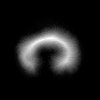
\includegraphics[width=0.9\textwidth]{fig/variational_dt}
      \caption{Image mobile}
      \label{subfig:variational_dt}
    \end{subfigure}%
    \begin{subfigure}[t]{0.33\textwidth}
      \centering
      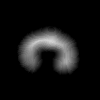
\includegraphics[width=0.9\textwidth]{fig/variational_dt3}
      \caption{Après déformation, sans MAJ}
      \label{subfig:variational_dt2}
    \end{subfigure}%
    \begin{subfigure}[t]{0.33\textwidth}
      \centering
      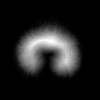
\includegraphics[width=0.9\textwidth]{fig/variational_dt2}
      \caption{Après déformation, avec MAJ}
      \label{subfig:variational_dt3}
    \end{subfigure}%

  \end{figure}
\end{frame}

\begin{frame}{Structures sans correspondance}
  Présence de \textbf{structures sans correspondance}.

  \alert{Structures sans correspondances} : régions d'une image -- fixe ou mobile -- absentes de l'autre image.

  \begin{figure}[ht]
    \centering
    \begin{subfigure}[t]{0.5\textwidth}
      \centering
      \includegraphics<1>[width=0.6\textwidth]{fig/overlay_dt_variational}%
      \includegraphics<2>[width=0.6\textwidth]{fig/overlay_dt_variational_circled}
      \caption{}
      \label{subfig:overlay_dt_variational}
    \end{subfigure}%
        \begin{subfigure}[t]{0.5\textwidth}
      \centering
      \includegraphics<1>[width=0.6\textwidth]{fig/overlay_dt_variational2}%
      \includegraphics<2>[width=0.6\textwidth]{fig/overlay_dt_variational2_circled}
      \caption{}
      \label{subfig:overlay_dt_variational2}
    \end{subfigure}%
  \end{figure}

  \vspace{-0.5cm}

\end{frame}

\begin{frame}{Recalage avec structures sans correspondance}


  Dans le domaine médical : recalage en présence de \textbf{lésions} ou de \textbf{tumeurs}.

  Recalage tenant compte des structures sans correspondance (\textbf{c}) \cite{Parisot_2012} :
  \begin{figure}[ht]
  \centering
  \begin{subfigure}[t]{0.33\textwidth}
    \centering 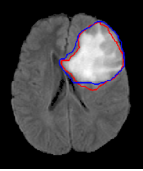
\includegraphics[width=0.9\textwidth]{fig/parisot_0}
    \caption{}
    \label{subfig:parisot_0}
  \end{subfigure}%
  \begin{subfigure}[t]{0.33\textwidth}
    \centering 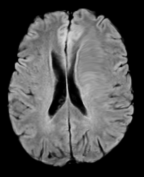
\includegraphics[width=0.9\textwidth]{fig/parisot_1}
    \caption{}
    \label{subfig:parisot_1}
  \end{subfigure}%
  \begin{subfigure}[t]{0.33\textwidth}
    \centering 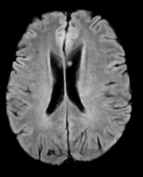
\includegraphics[width=0.9\textwidth]{fig/parisot_2}
    \caption{}
    \label{subfig:parisot_2}
  \end{subfigure}%
\end{figure}
  
\end{frame}

\begin{frame}{Recalage avec structures sans correspondance}
  \textbf{Principe :} verrouiller la position des pixels qui appartiennent à une structure sans correspondance.

  \textbf{Idée :} pondération de la métrique de similarité (\textit{via }\textbf{segmentation})
  
  $\Rightarrow$ Poids = 0 dans une structure sans correspondance et 1 sinon.

  \begin{figure}[ht]
    \centering
    \begin{subfigure}[t]{0.33\textwidth}
      \centering
      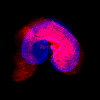
\includegraphics[width=0.9\textwidth]{fig/slice_overlay_affine}
      \caption{}
      \label{subfig:slice_overlay_affine}
    \end{subfigure}%
    \begin{subfigure}[t]{0.33\textwidth}
      \centering
      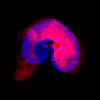
\includegraphics[width=0.9\textwidth]{fig/slice_overlay_0weight}
      \caption{}
      \label{subfig:slice_overlay_0weight}
    \end{subfigure}%

  \end{figure}

  \textbf{Problème :} pixels verrouillés.

\end{frame}


\begin{frame}{Recalage avec structures sans correspondance}
  Grain de blé : la déformation doit être \textbf{plus importante}
  dans les zones sans correspondance.

  \textbf{Travaux en cours :}

  \begin{enumerate}
  \item Identification des zones sans correspondance : utilisation du
    \textbf{champ de déformation}.
  \item Pondération de la métrique de similarité avec un \textbf{poids
      $> 1$} dans les zones sans correspondance.
  \end{enumerate}


\end{frame}

\begin{frame}{Champ de déformation}

  \textbf{Déterminant jacobien (c):} quantité reflétant les variations de volume du champ de vecteurs :
  \begin{itemize}
  \item $>1$ si agrandissement local (clair)
  \item $<1$ si rétrécissement local (sombre)
  \end{itemize}

  
  \begin{figure}[ht]
    \centering
    \begin{subfigure}[t]{0.33\textwidth}
      \centering
      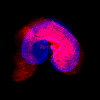
\includegraphics[width=0.9\textwidth]{fig/slice_overlay_affine}
      \caption{}
      \label{subfig:slice_overlay_affine}
    \end{subfigure}%
    \begin{subfigure}[t]{0.33\textwidth}
      \centering
      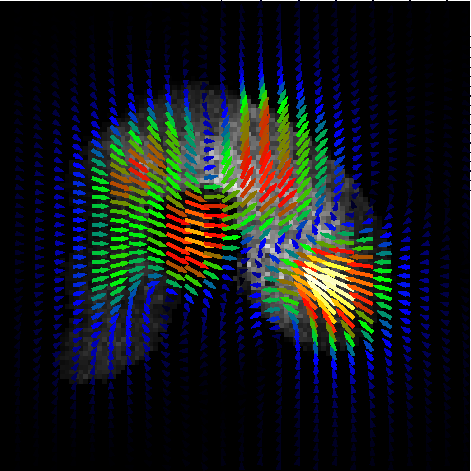
\includegraphics[width=0.9\textwidth]{fig/field_variational}
      \caption{}
      \label{subfig:field_variational}
    \end{subfigure}%
    \begin{subfigure}[t]{0.33\textwidth}
      \centering
      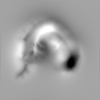
\includegraphics[width=0.9\textwidth]{fig/jacobien}
      \caption{}
      \label{subfig:jacobien}
    \end{subfigure}%

  \end{figure}
  \vspace{-0.3cm}
  $\Rightarrow$ structures sans correspondance = structures où le déterminant jacobien est $< 1$.

\end{frame}

\begin{frame}{Recalage sans correspondance}

  Pondération avec des \textbf{valeurs supérieures à 1} dans les zones sans correspondance.
  
  $\Rightarrow$ favorise leur déformation.

  \begin{figure}[ht]
    \centering
    \begin{subfigure}[t]{0.33\textwidth}
      \centering
      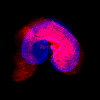
\includegraphics[width=0.9\textwidth]{fig/slice_overlay_affine}
      \caption{}
      \label{subfig:slice_overlay_affine}
    \end{subfigure}%
    \begin{subfigure}[t]{0.33\textwidth}
      \centering
      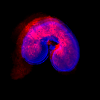
\includegraphics[width=0.9\textwidth]{fig/slice_overlay_ssdweight.png}
      \caption{}
      \label{subfig:field_variational}
    \end{subfigure}%
  \end{figure}
\end{frame}




\section{Analyse statistique}

\begin{frame}{Bruit}

  \textbf{Analyse statistique :} identifier les molécules dans les images MS dont la distribution corrèle avec celle de l'eau en IRM \vspace{0.2cm}.

  \textbf{Méthode employée :} corrélations trouvées \textbf{pixel à pixel} dans un espace réduit.

  \textbf{Problème :} images bruitées.

  \begin{figure}[ht]
    \centering
    \begin{subfigure}[t]{0.33\textwidth}
      \centering
      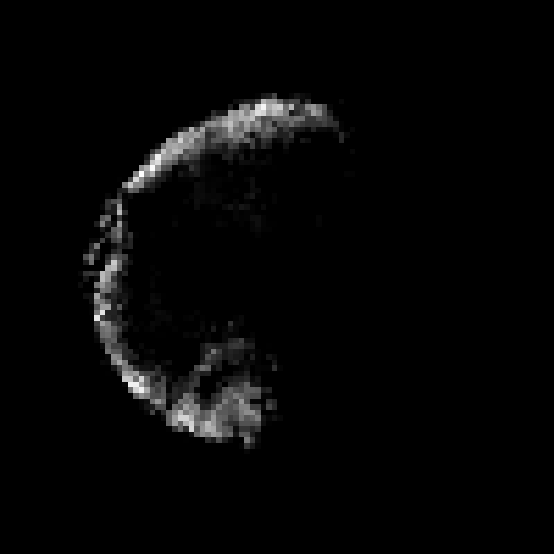
\includegraphics[width=0.9\textwidth]{fig/nmf_components_0}
      \caption{}
      \label{subfig:cluster0}
    \end{subfigure}%
     \begin{subfigure}[t]{0.33\textwidth}
      \centering
      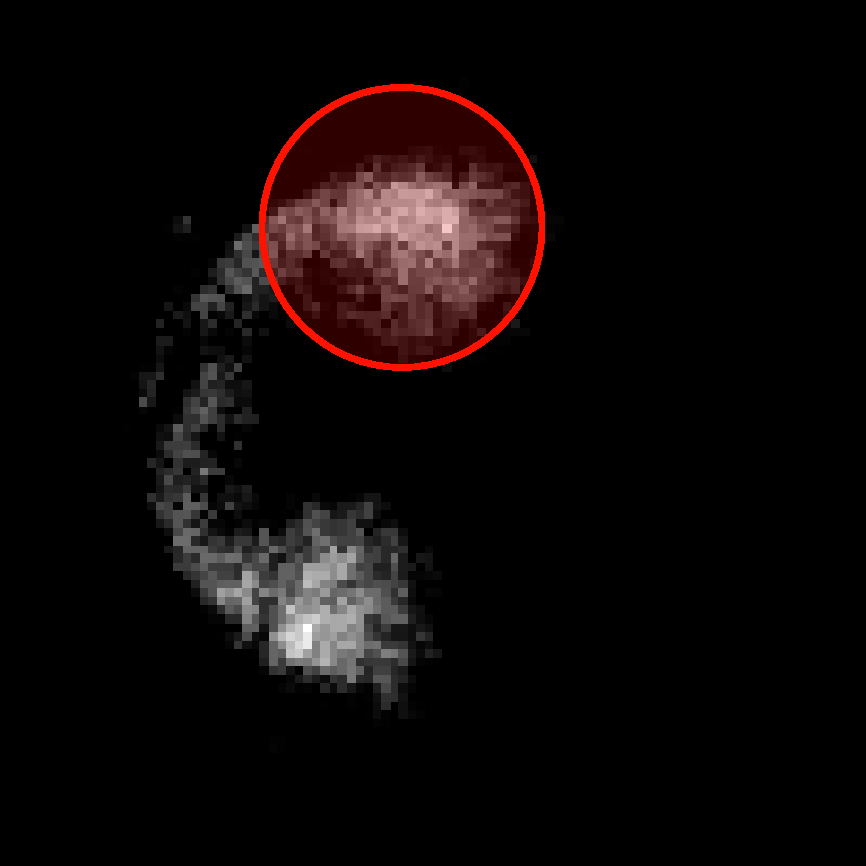
\includegraphics[width=0.9\textwidth]{fig/nmf_components_2_closeup}
      \caption{}
      \label{subfig:cluster2}
    \end{subfigure}%
     \begin{subfigure}[t]{0.33\textwidth}
      \centering
      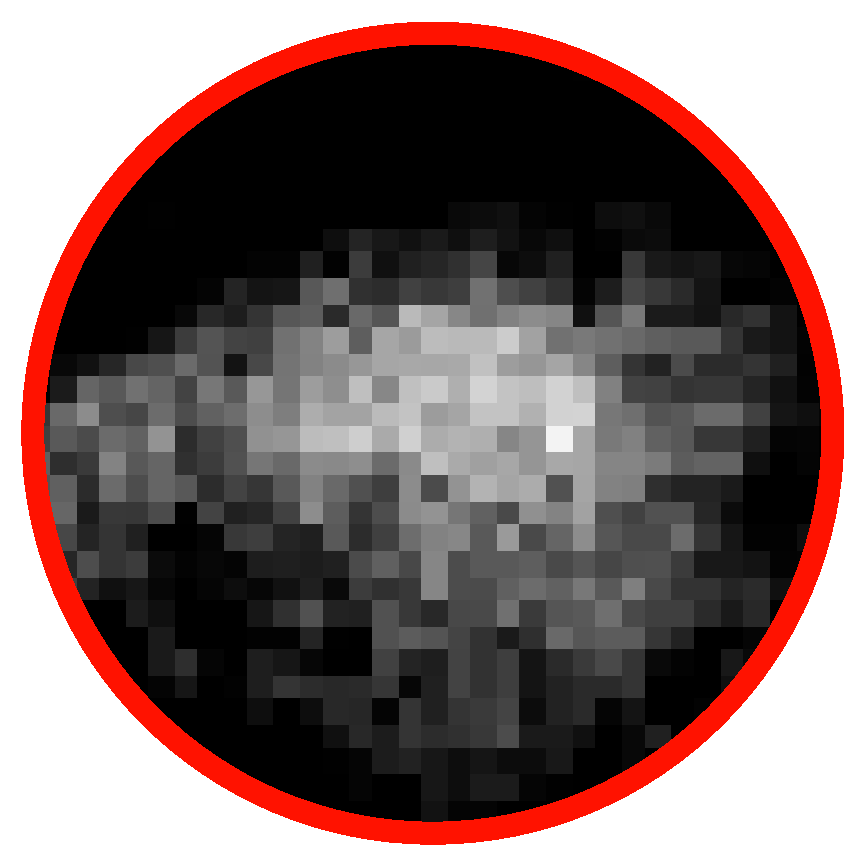
\includegraphics[width=0.90\textwidth]{fig/nmf_components_2_closeup2}
      \caption{}
      \label{subfig:cluster1}
    \end{subfigure}%
  \end{figure}

\end{frame}


\begin{frame}{Corrélations spatiales floues}
  \textbf{Idée :} considérer le \textbf{voisinage} du pixel pour s'abstraire du bruit

  $\Rightarrow$ méthodes \textbf{floues} \vspace{0.4cm}

  Papier de \cite{Alexandrov11} :

  \begin{figure}[ht]
    \centering
    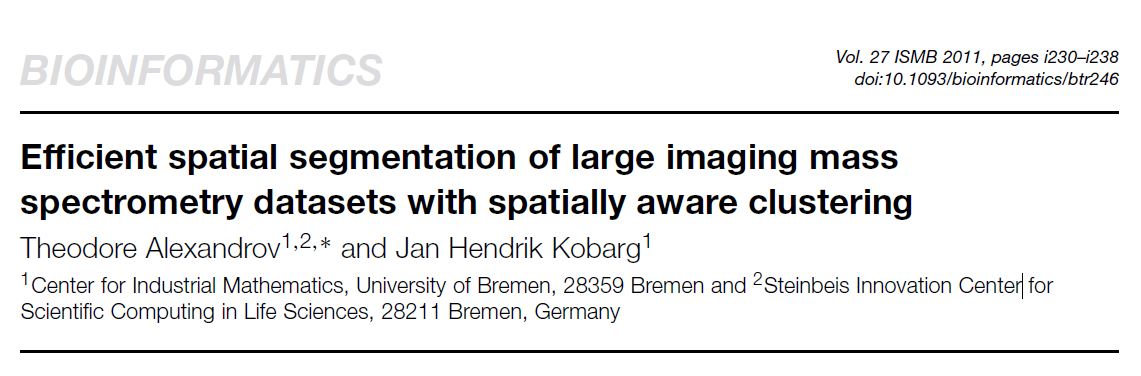
\includegraphics[width=0.9\textwidth]{fig/article_front}
    \caption{}
    \label{fig:article_front}
  \end{figure}
  
\end{frame}

\begin{frame}{Papier}
  \textbf{Contexte :} clustering de spectres dans une image MS.

  Exemple sur images de cerveau de rat:
  \begin{figure}[ht]
    \centering
    \begin{subfigure}[t]{0.33\textwidth}
      \centering
      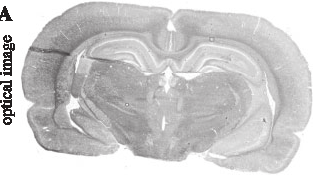
\includegraphics[width=0.9\textwidth]{fig/clustering_optical.pdf}
      \caption{}
      \label{subfig:clustering_optical.pdf}
    \end{subfigure}%
        \begin{subfigure}[t]{0.33\textwidth}
      \centering
      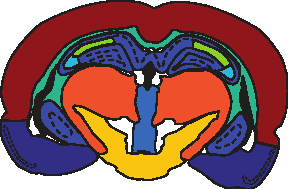
\includegraphics[width=0.9\textwidth]{fig/clustering_theoretical.pdf}
      \caption{}
      \label{subfig:clustering_th}
    \end{subfigure}%
        \begin{subfigure}[t]{0.33\textwidth}
      \centering
      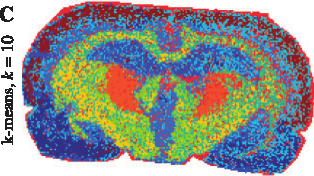
\includegraphics[width=0.9\textwidth]{fig/clustering_kmeans.pdf}
      \caption{}
      \label{subfig:clustering_kmeans}
    \end{subfigure}%
  \end{figure}

  $\Rightarrow$ Clustering classique insuffisant (cf. $k$-means, \textbf{(c)}).

  
\end{frame}

\begin{frame}{Clustering avec information spatiale}

  \textbf{Idée :} intégrer l'information spatiale des pixels dans un voisinage.
  
  \begin{itemize}
  \item Distance \textbf{``classique''} entre deux spectres : distance euclidienne.
  \item Distance \textbf{``au voisinage''} entre deux spectres : somme
    \textbf{pondérée} des distances euclidiennes entre chaque paire de spectre dans un \textbf{voisinage}.
  \end{itemize}



  \begin{figure}[ht]
    \centering
    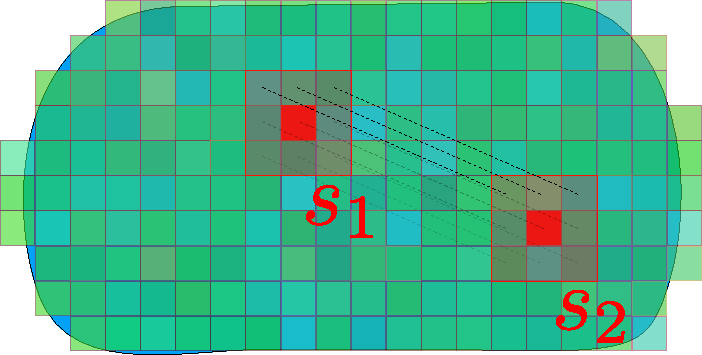
\includegraphics[width=0.45\textwidth]{fig/distance_pixels}
  \end{figure}

\end{frame}

% \begin{frame}{Représentation des données}
  
%   \textbf{Problème :} pour $n$ spectres: matrice de distances de taille $n^2$.

%   \textbf{Proposition :} représentation d'un spectre sous forme de vecteur comprenant son voisinage de rayon $r$, pondéré par la fonction $\alpha$:
%   \[
%     \Phi(s) = \left[ \alpha_{-r,-r} s(x-r, y-r),\ \dots,\ \alpha_{0,0} s(x, y),\ \dots,\ \alpha_{r,r} s(x+r, y+r) \right]
%   \]

%   $\Rightarrow$ la distance euclidienne entre deux vecteurs $\Phi(s_1)$ et $\Phi(s_2)$ correspond à la distance \textbf{``au voisinage''}.

%   \begin{figure}[ht]
%     \centering
%     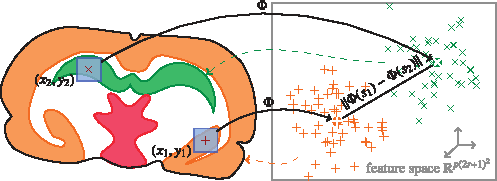
\includegraphics[width=0.6\textwidth]{fig/spectrum_projection}
%   \end{figure}

% \end{frame}

\begin{frame}{Pondération}
  Fonction de pondération : \textbf{fonction gaussienne}

  \begin{figure}[ht]
    \centering
    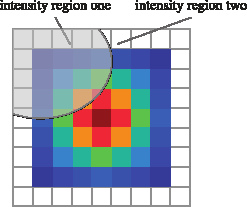
\includegraphics[width=0.35\textwidth]{fig/weights_gauss}
  \end{figure}

  \textbf{Structure de données :} on associe, à chaque point de l'image, son spectre et les spectres voisins pondérés.

\end{frame}


\begin{frame}{Algorithme}
  

  \textbf{Idée :} clustering en considérant les spectres et leur voisinage dans un espace réduit
  \begin{enumerate}
  \item Réduction de dimension des spectres par l'algorithme \textbf{FastMap}
  \item \textbf{Clustering} par l'algorithme des $k$-moyennes
  \end{enumerate}

\vspace{0.4cm}  

\textbf{FastMap} \cite{Faloutsos_1995} : transformation des points dans un espace réduit où les \textbf{distances sont préservées}.


\end{frame}

\begin{frame}{Importance de la normalisation}

  Facteur d'échelle :
  \begin{figure}[ht]
    \centering
    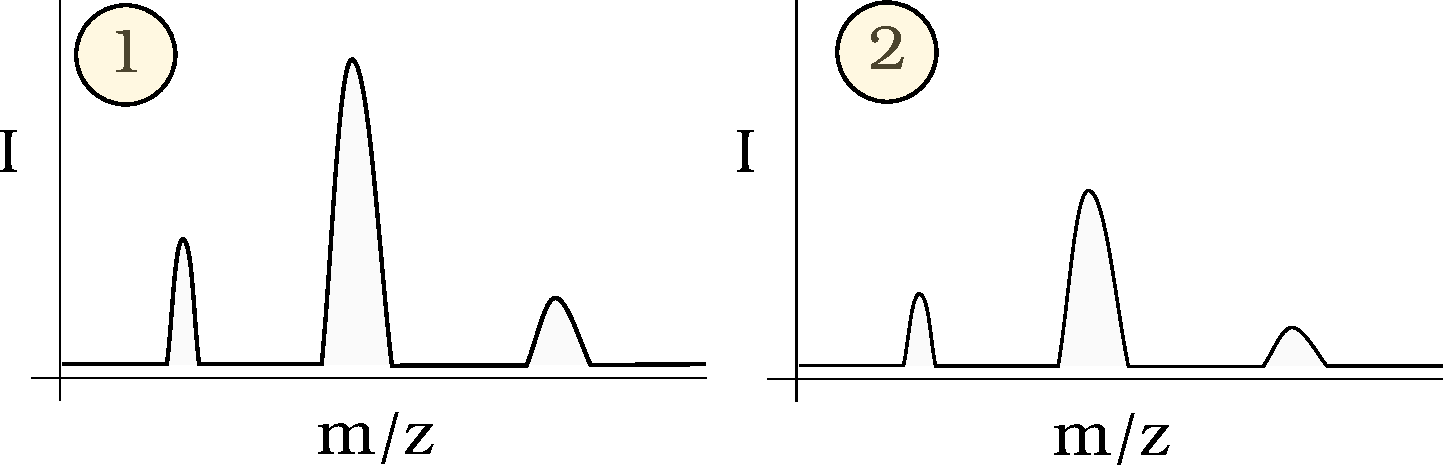
\includegraphics[width=0.9\textwidth]{fig/clustering_norm}
    \caption{}
    \label{fig:clustering_norm}
  \end{figure}
  
  \vspace{-0.5cm}
  $\Rightarrow$ distance euclidienne élevée : spectres considérés comme différents.

  Spectres \textbf{normalisés au préalable} : spectres considérés comme similaires.

\end{frame}



\begin{frame}{Résultats}
  \begin{figure}[ht]
    \centering
    \begin{subfigure}[t]{0.33\textwidth}
      \centering
      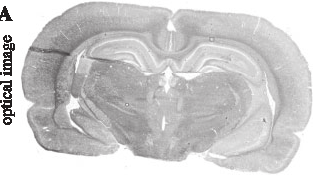
\includegraphics[width=0.9\textwidth]{fig/clustering_optical.pdf}
      \caption{Image optique}
      \label{subfig:clustering_optical.pdf}
    \end{subfigure}%
        \begin{subfigure}[t]{0.33\textwidth}
      \centering
      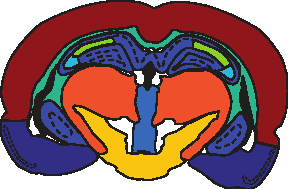
\includegraphics[width=0.9\textwidth]{fig/clustering_theoretical.pdf}
      \caption{Théorique}
      \label{subfig:clustering_th}
    \end{subfigure}%
        \begin{subfigure}[t]{0.33\textwidth}
      \centering
      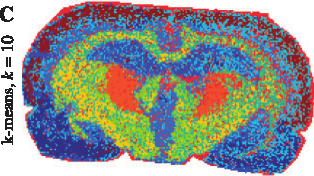
\includegraphics[width=0.9\textwidth]{fig/clustering_kmeans.pdf}
      \caption{$k$-means}
      \label{subfig:clustering_kmeans}
    \end{subfigure}
    \begin{flushright}
      \begin{subfigure}[t]{0.33\textwidth}
        \centering
        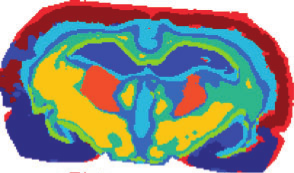
\includegraphics[width=0.9\textwidth]{fig/clustering_sa}
        \caption{$k$-means flou, gauss.}
        \label{subfig:clustering_sa}
      \end{subfigure}%
      \begin{subfigure}[t]{0.33\textwidth}
        \centering
        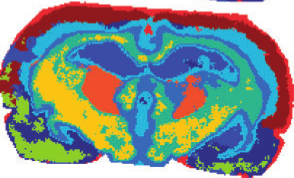
\includegraphics[width=0.9\textwidth]{fig/clustering_sasa}
        \caption{$k$-means flou, gauss. tronq.}
        \label{subfig:clustering_sasa}
      \end{subfigure}%

    \end{flushright}
  \end{figure}
\end{frame}

\begin{frame}{Résultats sur le grain de blé}
  \vspace{-0.2cm}
  Sans normalisation ($k=7$):

  \begin{figure}[ht]
    \centering
    \begin{subfigure}[t]{0.25\textwidth}
      \centering
      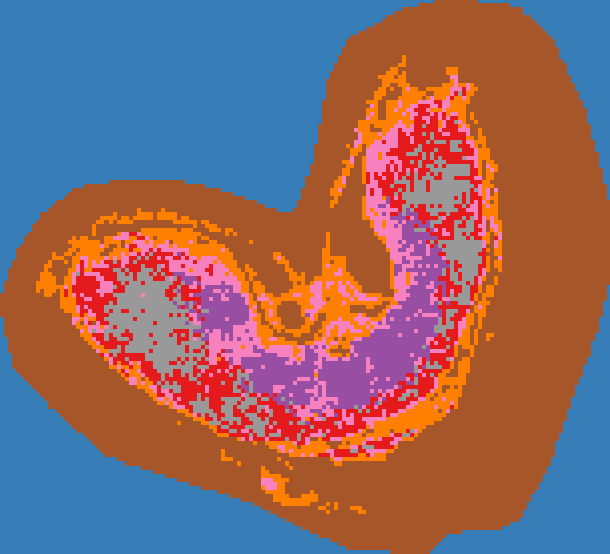
\includegraphics[width=0.95\textwidth]{fig/peaksel_prominence75_r0_full_colors}
      \caption{$r=0$}
      \label{subfig:peaksel_prominence75_r0_full_colors}
    \end{subfigure}%
    \begin{subfigure}[t]{0.25\textwidth}
      \centering
      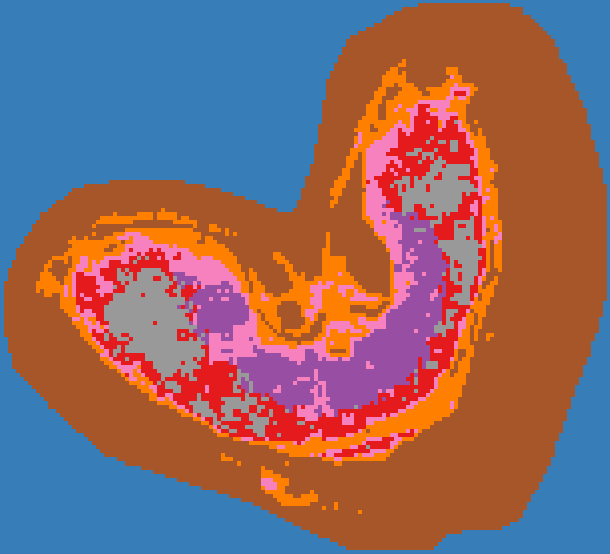
\includegraphics[width=0.95\textwidth]{fig/peaksel_prominence75_r1_full_colors}
      \caption{$r=1$}
      \label{subfig:peaksel_prominence75_r1_full_colors}
    \end{subfigure}%
    \begin{subfigure}[t]{0.25\textwidth}
      \centering
      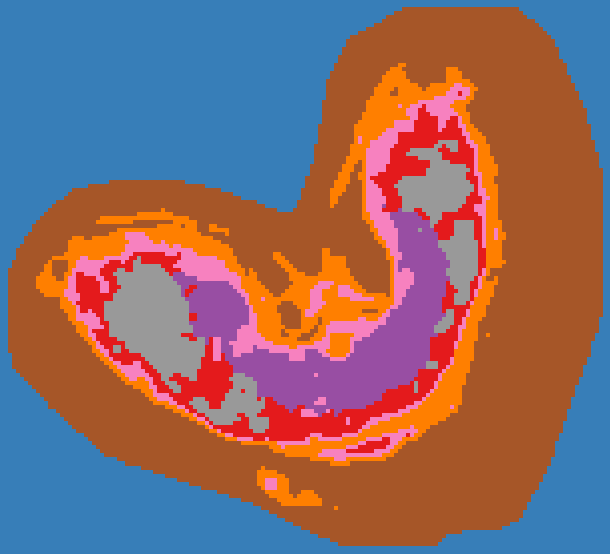
\includegraphics[width=0.95\textwidth]{fig/peaksel_prominence75_r2_full_colors}
      \caption{$r=2$}
      \label{subfig:peaksel_prominence75_r2_full_colors}
    \end{subfigure}%
    \begin{subfigure}[t]{0.25\textwidth}
      \centering
      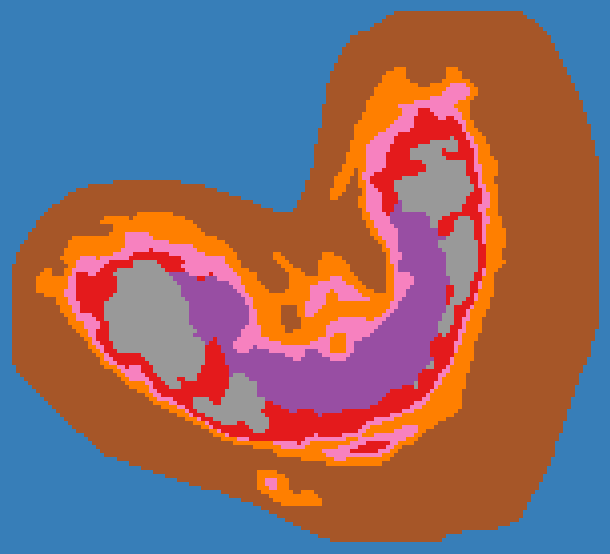
\includegraphics[width=0.95\textwidth]{fig/peaksel_prominence75_r3_full_colors}
      \caption{$r=3$}
      \label{subfig:peaksel_prominence75_r3_full_colors}
    \end{subfigure}%
    \begin{flushleft}
      \vspace{-0.2cm}
          Avec normalisation ($k=7$) :
    \end{flushleft}%
     \begin{subfigure}[t]{0.25\textwidth}
      \centering
      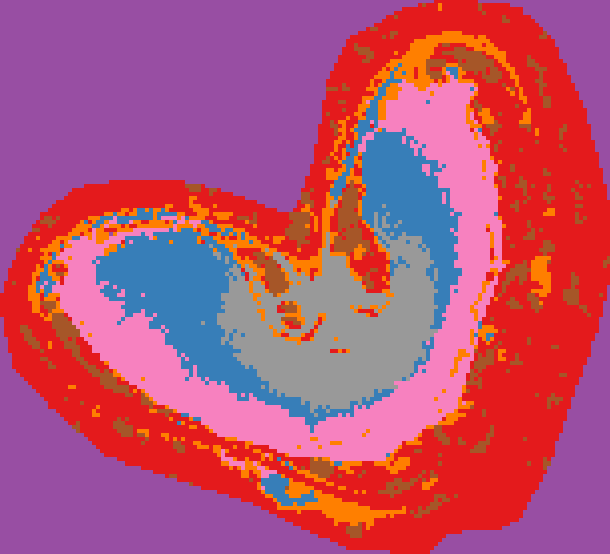
\includegraphics[width=0.95\textwidth]{fig/peaksel_prominence75_r0_full_norm_colors}
      \caption{$r=0$}
      \label{subfig:peaksel_prominence75_r0_full_norm_colors}
    \end{subfigure}%
    \begin{subfigure}[t]{0.25\textwidth}
      \centering
      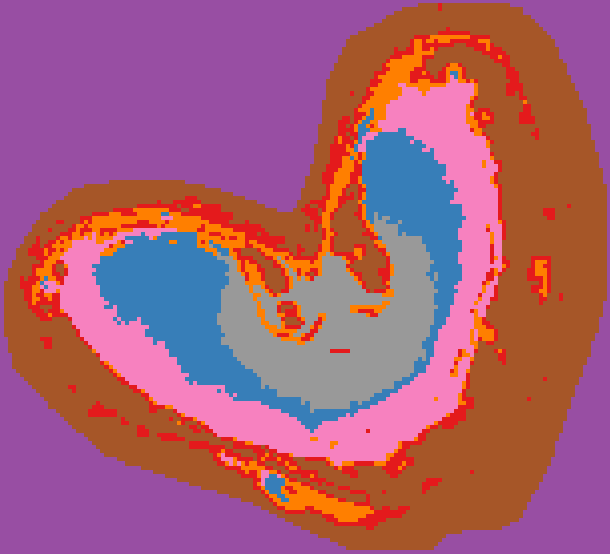
\includegraphics[width=0.95\textwidth]{fig/peaksel_prominence75_r1_full_norm_colors}
      \caption{$r=1$}
      \label{subfig:peaksel_prominence75_r1_full_norm_colors}
    \end{subfigure}%
    \begin{subfigure}[t]{0.25\textwidth}
      \centering
      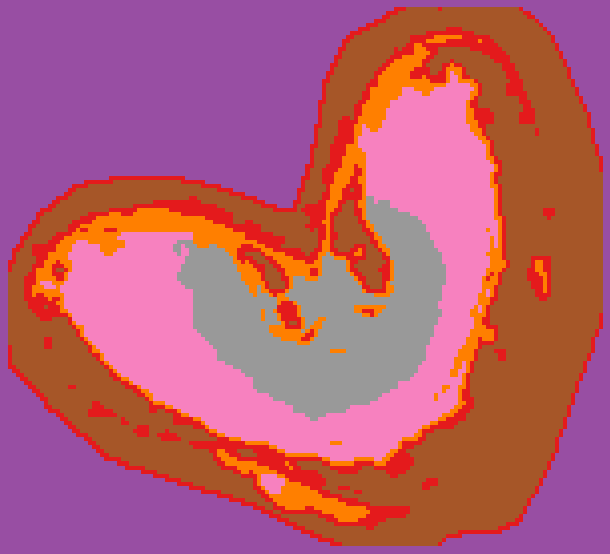
\includegraphics[width=0.95\textwidth]{fig/peaksel_prominence75_r2_full_norm_colors}
      \caption{$r=2$}
      \label{subfig:peaksel_prominence75_r2_full_norm_colors}
    \end{subfigure}%
    \begin{subfigure}[t]{0.25\textwidth}
      \centering
      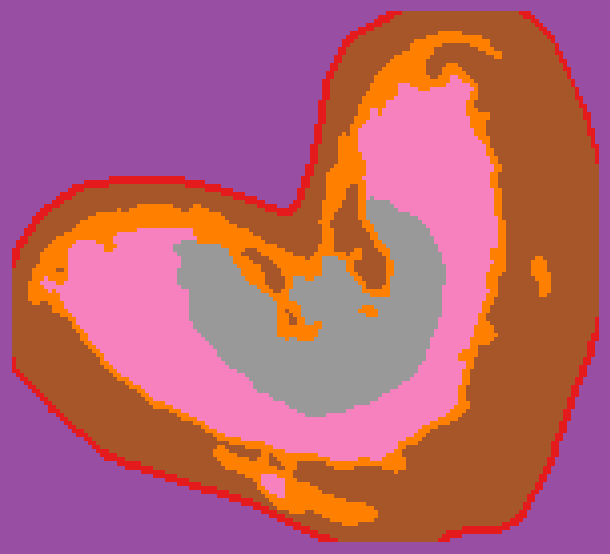
\includegraphics[width=0.95\textwidth]{fig/peaksel_prominence75_r3_full_norm_colors}
      \caption{$r=3$}
      \label{subfig:peaksel_prominence75_r3_full_norm_colors}
    \end{subfigure}

  \end{figure}

\end{frame}

\section{Traitement des images de blé Bobwhite}

\begin{frame}{Données}
  IRM :
  \begin{itemize}
  \item \textbf{Six stades} : 250, 350, 420, 500, 500, 580, 650DJ.
  \item \textbf{Six réplicats} par stade, en moyenne \textbf{14 coupes} par stade.
  \end{itemize}


  Imagerie MS :
  \begin{itemize}
  \item  \textbf{Trois stades} : 250, 500 et 650 DJ
  \item  \textbf{Deux réplicats} par stade, en moyenne \textbf{11 coupes} par stade.
  \item  \textbf{Deux enzymes} utilisées : xylanase et lichenase.
  \end{itemize}

Ici : \textbf{un seul grain} étudié pour les stades 250, 500 et 650 DJ.

\end{frame}

\begin{frame}{Traitement des images IRM}

  \begin{enumerate}
  \item \textbf{Débruitage}
  \item \textbf{Image en densité} $\Rightarrow$ premier écho.
  \item Ajustement d'une fonction mono-exponentielle par moindres carrés $\Rightarrow$ \textbf{image en $T_2^*$}.
  \item \textbf{Segmentation} : plus grande composante connexe
  \end{enumerate}

  \begin{figure}[ht]
    \centering
    \begin{subfigure}[t]{0.33\textwidth}
      \centering
      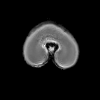
\includegraphics[width=0.9\textwidth]{fig/irm_250_density_s6}
      \caption{}
      \label{subfig:irm_250_density_s6}
    \end{subfigure}%
    \begin{subfigure}[t]{0.33\textwidth}
      \centering
      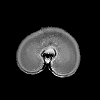
\includegraphics[width=0.9\textwidth]{fig/irm_500_density_s5}
      \caption{}
      \label{subfig:irm_500_density_s5}
    \end{subfigure}%
    \begin{subfigure}[t]{0.33\textwidth}
      \centering
      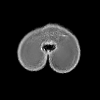
\includegraphics[width=0.9\textwidth]{fig/irm_650_density_s8}
      \caption{}
      \label{subfig:irm_650_density_s8}
    \end{subfigure}%
  \end{figure}


\end{frame}

\begin{frame}{Traitement des images MS}
  \begin{enumerate}
  \item \textbf{Normalisation} par le SIC
  \item \textbf{Sélection de pics} basée sur la prominence locale
  \item \textbf{Réalignement} des pics
  \item \textbf{Clustering} avec normalisation des spectres \cite{Alexandrov11}
  \item[4b.] \textbf{Segmentation} par la mesure de cohérence spatiale
  \end{enumerate}

        \begin{figure}[ht]
    \centering
    \begin{subfigure}[t]{0.33\textwidth}
      \centering
      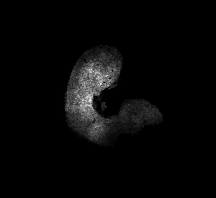
\includegraphics[width=0.9\textwidth]{fig/maldi_250_density_s6}
      \caption{}
      \label{subfig:maldi_250_density_s6}
    \end{subfigure}%
    \begin{subfigure}[t]{0.33\textwidth}
      \centering
      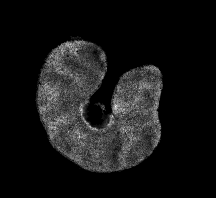
\includegraphics[width=0.9\textwidth]{fig/maldi_500_density_s5}
      \caption{}
      \label{subfig:maldi_500_density_s5}
    \end{subfigure}%
    \begin{subfigure}[t]{0.33\textwidth}
      \centering
      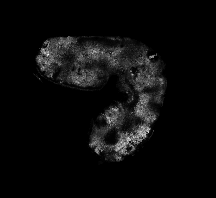
\includegraphics[width=0.9\textwidth]{fig/maldi_650_density_s8}
      \caption{}
      \label{subfig:maldi_650_density_s8}
    \end{subfigure}%
  \end{figure}
\end{frame}

\begin{frame}{Clustering des images MS}
  
  \textbf{Xylanase}, stade 250 DJ :
    \begin{itemize}
    \item \textbf{Haut du grain (brosse) }: arabinoxylanes (AX) avec un degré de polymérisation (DP) variable, proche de 10, sans modification.
    \item \textbf{Milieu--bas du grain (vers embryon)}
      \begin{itemize}
      \item Sur le pourtour du grain \textbf{(a)}: AX avec faibles DP (5--10), avec acétylations (de 1 à 3).
      \item Proche cavité \textbf{(b)}: AX DP de 9 à 11, sans modification.
      \item Embryon \textbf{(c)}: AX 4--9 sans modification.
      \end{itemize}
    \end{itemize}

    \begin{figure}[ht]
      \centering
      \begin{subfigure}[t]{0.25\textwidth}
        \centering
        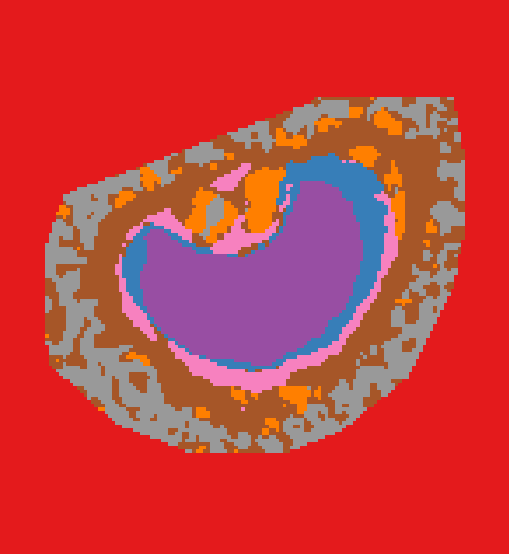
\includegraphics[width=0.9\textwidth]{fig/clustering_250Xyl_s1.png}
        \caption{}
        \label{subfig:clustering_250Xyl_s1.png}
      \end{subfigure}%
      \begin{subfigure}[t]{0.25\textwidth}
        \centering
        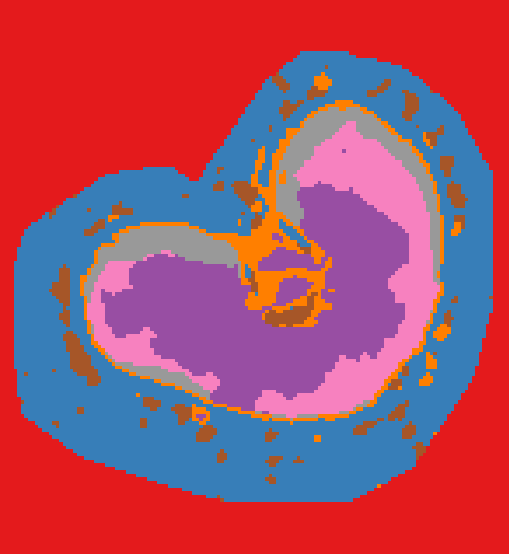
\includegraphics[width=0.9\textwidth]{fig/clustering_250Xyl_s5.png}
        \caption{}
        \label{subfig:clustering_250Xyl_s5.png}
      \end{subfigure}%
      \begin{subfigure}[t]{0.25\textwidth}
        \centering
        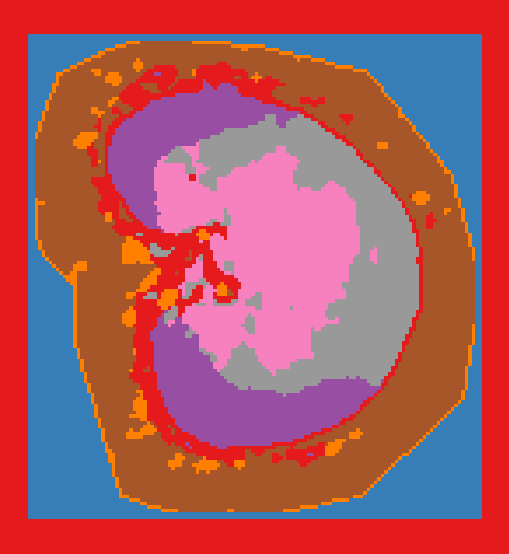
\includegraphics[width=0.9\textwidth]{fig/clustering_250Xyl_s12.png}
        \caption{}
        \label{subfig:clustering_250Xyl_s12.png}
      \end{subfigure}%

    \end{figure}




\end{frame}


\begin{frame}{Clustering des images MS}
  \begin{columns}
    \begin{column}{.7\textwidth}
       \textbf{Xylanase}, stades\textbf{ 500 et 650 DJ} \textbf{(a)}: AX de DP 6 à 10, sans modification chimique, répartis uniformément dans le grain.

      \vspace{1.5cm}

      \textbf{Lichenase,} stades \textbf{250, 500 et 650 DJ} \textbf{(b)}: BG DP 3-4-5  (moins fréquemment BG 6 pour les trois stades, et BG 2 pour le stade 650DJ).
    \end{column}

    \begin{column}{.3\textwidth}
      \begin{figure}[ht] 
       \centering
        \begin{subfigure}[t]{0.99\textwidth}
          \centering
          \includegraphics[width=0.9\textwidth]{fig/clustering_500Xyl_s5.png}
          \caption{}
          \label{subfig:clustering500Xyl}
        \end{subfigure}
        \begin{subfigure}[t]{0.99\textwidth}
          \centering
          \includegraphics[width=0.9\textwidth]{fig/clustering_250Lich_s6.png}
          \caption{}
          \label{subfig:clustering_250Lich_s6.png}
        \end{subfigure}%

      \end{figure}

    \end{column}
  \end{columns}


\end{frame}

\begin{frame}{Recalage}

  Deux étapes :
  \begin{enumerate}
  \item \textbf{Affine} sur la transformée en distance
  \item \textbf{Variationnel} sur la transformée en distance, sans prise en compte des structures sans correspondance
  \end{enumerate}

  $\Rightarrow$ La précision du recalage est \textbf{variable} en fonction de la coupe.
\end{frame}

\begin{frame}{Recalage}
Proportions de pixels en commun (en \%):
\begin{table}[]
\begin{tabular}{lllllll}
\hline
                            & \multicolumn{2}{l}{250} & \multicolumn{2}{l}{500} & \multicolumn{2}{l}{650} \\ \hline
       & Xyl        & Lich       & Xyl        & Lich       & Xyl        & Lich       \\ \hline
Affine & 84.6      & 87.4      & 85.3      & 84.0      & 86.7      & 86.5      \\
Variationnel                 & 91.4      & 92.8      & 91.9      & 89.2      & 92.0      & 92.8      \\ \hline
\end{tabular}
\end{table}

\underline{Exemple :} Stade 500 DJ, Xylanase
  \begin{figure}[ht]
    \centering
    \begin{subfigure}[t]{0.33\textwidth}
      \centering
      \includegraphics[width=0.9\textwidth]{fig/recalage_500Xyl_0}
      \caption{}
      \label{subfig:recalage_500Xyl_0}
    \end{subfigure}%
    \begin{subfigure}[t]{0.33\textwidth}
      \centering
      \includegraphics[width=0.9\textwidth]{fig/recalage_500Xyl_2}
      \caption{}
      \label{subfig:recalage_500Xyl_2}
    \end{subfigure}%
    \begin{subfigure}[t]{0.33\textwidth}
      \centering
      \includegraphics[width=0.9\textwidth]{fig/recalage_500Xyl_8}
      \caption{}
      \label{subfig:recalage_500Xyl_8}
    \end{subfigure}%
  \end{figure}


\end{frame}

\begin{frame}{Analyse statistique}
  
  Deisotoping, puis réduction de dimension par NMF.
  \begin{itemize}
  \item 3 grains $\times$ 2 enzymes $\times$ 2 informations en IRM $\times$ 2 choix de dimensions (2D ou 3D) $\times$ 2 conditions d'analyse (rapports) = \textbf{48} sources de données à traiter.
    
    $\Rightarrow$ protocole pour une analyse rigoureuse.
  \end{itemize}
  
  \textbf{Protocole d'analyse :}
  \begin{enumerate}
  \item Analyse \textbf{complète} des résultats en \textbf{3D}
  \item Analyse \textbf{sélective} des résultats en \textbf{2D}: pertinence des coupes en fonction de :
    \begin{enumerate}
    \item la précision du recalage
    \item la précision de la reconstruction de l'image IRM par les composantes de la NMF
    \end{enumerate}
  \end{enumerate}

\end{frame}


\begin{frame}{Stade 250 DJ, Xylanase}
  \textbf{Densité}
  
  \textbf{En 3D :}
    \vspace{-0.4cm}

    \begin{table}[]
    \centering
    \begin{adjustbox}{max width=1\textwidth}
      \begin{tabular}{llllllllllllllll}
        \toprule
        Ordre & 1       & 2       & 3       & 4       & 5       & 6       & 7       & 8       & 9       & 10       \\
        \midrule
        m/z & 701.3 & 611.26 & 609.38 & 653.24 & 743.3 & 785.32 & 650.55 & 875.33 & 1007.41 & 780.83 \\
        Annotation & AX5 1.Ac & AX4 1.Ac & ? & AX4 2.Ac & AX 5 1.Ac & AX5 2.Ac & ? & AX6 1.Ac & ? & ? \\
        \bottomrule
      \end{tabular}
    \end{adjustbox}
  \end{table}

  \textbf{En 2D :} résultats sensiblement identiques.

  \begin{figure}[ht]
    \centering
    \begin{subfigure}[t]{0.33\textwidth}
      \centering
      \includegraphics[width=0.9\textwidth]{fig/stats_250Xyl_density_irm}
    \end{subfigure}%
    \begin{subfigure}[t]{0.33\textwidth}
      \centering
      \includegraphics[width=0.9\textwidth]{fig/stats_250Xyl_density}
    \end{subfigure}%
    
  \end{figure}

  
\end{frame}

\begin{frame}{Stade 250 DJ, Xylanase}
  \textbf{$T_2^*$}

  \textbf{En 3D:}
  \vspace{-0.4cm}
  \begin{table}[]
    \centering
    \begin{adjustbox}{max width=1\textwidth}
      \begin{tabular}{llllllllllllllll}
        \toprule
        Ordre & 1       & 2       & 3       & 4       & 5       & 6       & 7       & 8       & 9       & 10       \\
        \midrule
        m/z &    743.3 & 965.38 & 1097.44 & 1265.46 & 1223.45 & 963.65 & 1133.43 & 875.33 & 1139.41 & 1271.45 \\
        Annotation & AX5 1.Ac & AX7 & AX8 & AX8 4.Ac & AX8 3.Ac & ? & AX7 4.Ac & AX6 1.Ac & AX8 1.Ac & AX9 1.Ac \\
        \bottomrule
      \end{tabular}
    \end{adjustbox}
  \end{table}

  \textbf{En 2D :} résultats différents, similaires à ceux obtenus pour l'\textbf{image en densité}.

    \begin{figure}[ht]
    \centering
    \begin{subfigure}[t]{0.33\textwidth}
      \centering
      \includegraphics[width=0.9\textwidth]{fig/stats_250Xyl_t2_irm}
    \end{subfigure}%
    \begin{subfigure}[t]{0.33\textwidth}
      \centering
      \includegraphics[width=0.9\textwidth]{fig/stats_250Xyl_t2}
    \end{subfigure}%
    
  \end{figure}

  
\end{frame}

\begin{frame}{Stade 250 DJ, Lichenase}
    \textbf{Densité}
  
    \textbf{En 3D :}
    \vspace{-0.4cm}
    \begin{table}[]
    \centering
    \begin{adjustbox}{max width=1\textwidth}
      \begin{tabular}{llllllllllllllll}
        \toprule
        Ordre & 1       & 2       & 3       & 4       & 5       & 6       & 7       & 8       & 9       & 10       \\
        \midrule
        m/z &   526.81 & 688.73 & 527.16 & 689.2 & 808.67 & 803.82 & 803.19 & 689.33 & 680.97 & 945.2 \\
        Annotation &  ? & ? & BG3 & BG4 & ? & ? & ? & ? & ? & ?\\
        \bottomrule
      \end{tabular}
    \end{adjustbox}
  \end{table}



  \textbf{En 2D :} BG2 et 3 principalement + AX (très variable selon coupe)

  \begin{figure}[ht]
    \centering
    \begin{subfigure}[t]{0.33\textwidth}
      \centering
      \includegraphics[width=0.9\textwidth]{fig/stats_250Xyl_density_irm}
    \end{subfigure}%
    \begin{subfigure}[t]{0.33\textwidth}
      \centering
      \includegraphics[width=0.9\textwidth]{fig/stats_250Lich_density}
    \end{subfigure}%
    
  \end{figure}
\end{frame}

\begin{frame}{Stade 250 DJ, Lichenase}
  $T_2^*$

  \textbf{En 3D :}
  \vspace{-0.4cm}
    \begin{table}[]
    \centering
    \begin{adjustbox}{max width=1\textwidth}
      \begin{tabular}{llllllllllllllll}
        \toprule
        Ordre & 1       & 2       & 3       & 4       & 5       & 6       & 7       & 8       & 9       & 10       \\
        \midrule
        m/z &     1097.38 & 851.33 & 965.17 & 852.11 & 853.23 & 1097.28 & 1229.4 & 1013.36 & 689.33 & 1175.42 \\
        Annotation &  BG6 2.Ac & BG5 & AX7 & ? & AX3 K+ MeGlcA 5.Ac & AX8 & AX9 & BG6 & BG4 & BG7\\
        \bottomrule
      \end{tabular}
    \end{adjustbox}
  \end{table}




  \textbf{En 2D :} BG2 et 3 avec acétylations

  \begin{figure}[ht]
    \centering
    \begin{subfigure}[t]{0.33\textwidth}
      \centering
      \includegraphics[width=0.9\textwidth]{fig/stats_250Xyl_density_irm}
    \end{subfigure}%
    \begin{subfigure}[t]{0.33\textwidth}
      \centering
      \includegraphics[width=0.9\textwidth]{fig/stats_250Lich_t2}
    \end{subfigure}%
    
  \end{figure}
  
\end{frame}

\begin{frame}{Stade 500 DJ, Xylanase}
  \textbf{Densité}

  \textbf{En 3D :}
  \vspace{-0.4cm}
    \begin{table}[]
    \centering
    \begin{adjustbox}{max width=1\textwidth}
      \begin{tabular}{llllllllllllllll}
        \toprule
        Ordre & 1       & 2       & 3       & 4       & 5       & 6       & 7       & 8       & 9       & 10       \\
        \midrule
        m/z &   611.21 & 735.35 & 743.23 & 732.68 & 732.75 & 569.18 & 875.41 & 1007.48 & 999.69 & 999.6 \\  
        Annotation &  AX4 1.Ac & ? & AX5 1.Ac & ? & ? & AX4 & ? & ? & ? & ?\\
        \bottomrule
      \end{tabular}
    \end{adjustbox}
  \end{table}

  \textbf{En 2D :} AX7 à 9, de 1 à 7 Ac

  \begin{figure}[ht]
    \centering
    \begin{subfigure}[t]{0.33\textwidth}
      \centering
      \includegraphics[width=0.9\textwidth]{fig/stats_500Xyl_density_irm}
    \end{subfigure}%
    \begin{subfigure}[t]{0.33\textwidth}
      \centering
      \includegraphics[width=0.9\textwidth]{fig/stats_500Xyl_density}
    \end{subfigure}%
    
  \end{figure}
  

 
\end{frame}

\begin{frame}{Stade 500 DJ, Xylanase}
  $T_2^*$
  
  \textbf{En 3D :}
  \vspace{-0.4cm}
    \begin{table}[]
    \centering
    \begin{adjustbox}{max width=1\textwidth}
      \begin{tabular}{llllllllllllllll}
        \toprule
        Ordre & 1       & 2       & 3       & 4       & 5       & 6       & 7       & 8       & 9       & 10       \\
        \midrule
        m/z &   611.21 & 735.35 & 743.23 & 732.68 & 732.75 & 999.69 & 999.6 & 1139.38 & 1259.56 & 1007.36 \\
        Annotation &  AX4 1.Ac & ? & AX5 1.Ac & ? & ? & ? & ? & AX8 1.Ac & ? & AX7 1.Ac\\
        \bottomrule
      \end{tabular}
    \end{adjustbox}
  \end{table}




  \textbf{En 2D :} similaire + AX5 à 7 avec DP $\geq 5$

  \begin{figure}[ht]
    \centering
    \begin{subfigure}[t]{0.33\textwidth}
      \centering
      \includegraphics[width=0.9\textwidth]{fig/stats_500Xyl_t2}
    \end{subfigure}%
    \begin{subfigure}[t]{0.33\textwidth}
      \centering
      \includegraphics[width=0.9\textwidth]{fig/stats_500Xyl_t2_irm}
    \end{subfigure}%
    
  \end{figure}
\end{frame}



%% Lichenase 500 densité
\begin{frame}{Stade 500 DJ, Lichenase}
  \textbf{Densité}
  
  \textbf{En 3D :}
  \vspace{-0.4cm}
    \begin{table}[]
    \centering
    \begin{adjustbox}{max width=1\textwidth}
      \begin{tabular}{llllllllllllllll}
        \toprule
        Ordre & 1       & 2       & 3       & 4       & 5       & 6       & 7       & 8       & 9       & 10       \\
        \midrule
        m/z &   831.14 & 951.18 & 2021.62 & 2021.83 & 2022.74 & 1889.78 & 1889.57 & 2153.81 & 1757.53 & 852.67 \\
        Annotation &  BG4 K+ 3.Ac & BG5 K+ 2.Ac & AX15 & ? & ? & AX14 & ? & BG12 4.Ac & AX13 & ?\\
        \bottomrule
      \end{tabular}
    \end{adjustbox}
  \end{table}


  \textbf{En 2D :} similaire

  \begin{figure}[ht]
    \centering
    \begin{subfigure}[t]{0.33\textwidth}
      \centering
      \includegraphics[width=0.9\textwidth]{fig/stats_500Lich_density_irm}

      
    \end{subfigure}%
    \begin{subfigure}[t]{0.33\textwidth}
      \centering
      \includegraphics[width=0.9\textwidth]{fig/stats_500Lich_density}

    \end{subfigure}%
    
  \end{figure}
\end{frame}

\begin{frame}{Stade 500 DJ, Lichenase}
  \textbf{$T_2^*$}

  
  \textbf{En 3D :}
  \vspace{-0.4cm}
    \begin{table}[]
    \centering
    \begin{adjustbox}{max width=1\textwidth}
      \begin{tabular}{llllllllllllllll}
        \toprule
        Ordre & 1       & 2       & 3       & 4       & 5       & 6       & 7       & 8       & 9       & 10       \\
        \midrule
        m/z &     2021.62 & 1889.57 & 1889.78 & 951.18 & 2021.83 & 1757.53 & 2022.74 & 2153.81 & 831.14 & 1757.73 \\
        Annotation &  AX15 & AX14 & ? & BG5 K+ 2.Ac & ? & AX13 & ? & BG12 4.Ac & BG4 K+ 3Ac & AX13\\
        \bottomrule
      \end{tabular}
    \end{adjustbox}
  \end{table}


  \textbf{En 2D :} BG 2--3, K+, 2.Ac

  \begin{figure}[ht]
    \centering
    \begin{subfigure}[t]{0.33\textwidth}
      \centering
      \includegraphics[width=0.9\textwidth]{fig/stats_500Lich_t2_irm}

      
    \end{subfigure}%
    \begin{subfigure}[t]{0.33\textwidth}
      \centering
      \includegraphics[width=0.9\textwidth]{fig/stats_500Lich_t2}

    \end{subfigure}%
    
  \end{figure}
\end{frame}


\begin{frame}{Stade 650 DJ, Xylanase}
  \textbf{Densité}
  
  \textbf{En 3D :}
  \vspace{-0.4cm}
    \begin{table}[]
    \centering
    \begin{adjustbox}{max width=1\textwidth}
      \begin{tabular}{llllllllllllllll}
        \toprule
        Ordre & 1       & 2       & 3       & 4       & 5       & 6       & 7       & 8       & 9       & 10       \\
        \midrule
        m/z &     701.22 & 965.3 & 834.09 & 965.51 & 965.09 & 833.26 & 1097.34 & 1098.1 & 827.56 & 1229.48 \\
        Annotation &  AX5 & AX7 & ? & ? & ? & AX6 & AX8 & ?  & ? & AX9\\
        \bottomrule
      \end{tabular}
    \end{adjustbox}
  \end{table}


  \textbf{En 2D :} similaire

  \begin{figure}[ht]
    \centering
    \begin{subfigure}[t]{0.33\textwidth}
      \centering
      \includegraphics[width=0.9\textwidth]{fig/stats_500Lich_density_irm}

      
    \end{subfigure}%
    \begin{subfigure}[t]{0.33\textwidth}
      \centering
      \includegraphics[width=0.9\textwidth]{fig/stats_500Lich_density}

    \end{subfigure}%
    
  \end{figure}
\end{frame}



\section{Bilan}

\begin{frame}{Bilan}

  Chaîne de traitement \textbf{ajustée} pour le \textbf{traitement automatique} d'images 3D.

  Résultats \textbf{préliminaires} au stade 250 DJ: confirment les \textbf{résultats précédents}.

  \vspace{0.4cm}

  Perspectives:
  \begin{itemize}
  \item Amélioration du recalage : \textbf{vérification} de la segmentation + \textbf{structures sans correspondance}
  \item Analyse statistique avec normalisation des spectres (\textbf{norme euclidienne})
  \item \textbf{Automatiser} l'analyse sélective en 2D
  \end{itemize}


\end{frame}




\appendix
\setbeamertemplate{headline}{%
  % \nointerlineskip
  % \begin{beamercolorbox}[wd=\paperwidth,leftskip=0.5cm,ht=0pt,dp=0pt]{block title}%
  %   \usebeamerfont{page number in head/foot}{\insertsection}
  % \end{beamercolorbox}%
  % \if@useTitleProgressBar
  % \nointerlineskip
  % % \vspace{-0.7cm}
  % \begin{beamercolorbox}[wd=\paperwidth,ht=0pt,dp=5pt]{section}
  %   \progressbar@titleprogressbar
  % \end{beamercolorbox}
  % \fi
  % \nointerlineskip
}

% \setbeamertemplate{frametitle}{%
%   \begin{beamercolorbox}[wd=\paperwidth,leftskip=0.7cm,rightskip=0.3cm,ht=0pt,dp=0pt]{frametitle}
%     \usebeamerfont{frametitle}\MakeLowercase{\protect\insertframetitle}
%   \end{beamercolorbox}
% }

\begin{frame}[allowframebreaks]
  \frametitle{Références}
  \setbeamertemplate{bibliography item}{$\bullet$}
  \bibliographystyle{apalike}
  \scriptsize{
    \bibliography{main}
  }
\end{frame}

\section{Ajustement de fonctions exponentielles}
% \begin{frame}{Ajustement de fonctions exponentielles}
  
%   \textbf{Précédemment}: trop peu d'échos $\Rightarrow$ surajustement, décroissance incomplète

%   \begin{figure}[ht]
%     \centering
%     \begin{subfigure}[t]{0.5\textwidth}
%       \centering
%       \includegraphics[width=0.8\textwidth]{fig/wrongfit_overfitting}
%       \caption{Surajustement}
%       \label{subfig:wrongfit_overfitting}
%     \end{subfigure}%
%     \begin{subfigure}[t]{0.5\textwidth}
%       \centering
%       \includegraphics[width=0.8\textwidth]{fig/wrongfit_missing}
%       \caption{Décroissance incomplète}
%       \label{subfig:wrongfit_missing}
%     \end{subfigure}%

%   \end{figure}


%   Nouvelles images: \textbf{plus d'échos} (8 $\rightarrow$ 16)

%   \underline{Objectif :} modélisation \textbf{plus précise} de la décroissance du signal  
% \end{frame}

% \begin{frame}{Ajustement par morceaux}
%   Modélisation par une \textbf{somme de fonctions exponentielles} (bi-exponentielle)

%   Ajustement de \textbf{deux droites} sur le logarithme des intensités \textbf{par morceaux} :

%   \begin{figure}[ht]
%     \centering
%     \begin{subfigure}[t]{0.5\textwidth}
%       \centering
%       \includegraphics<1-3>[width=0.95\textwidth]{fig/biexponential}%
%       \includegraphics<4>[width=0.95\textwidth]{fig/biexponential_fitted}%
%       \caption{Intensités}
%       \label{subfig:}
%     \end{subfigure}%
%     \onslide<2->
%     \begin{subfigure}[t]{0.5\textwidth}
%       \centering
%       \includegraphics<2>[width=0.95\textwidth]{fig/biexponential_log}%
%       \includegraphics<3->[width=0.95\textwidth]{fig/biexponential_log_piecewise}
%       \caption{Log des intensités}
%       \label{subfig:}
%     \end{subfigure}%
%   \end{figure}

% \end{frame}

% \begin{frame}{Ajustement par morceaux}
%   \textbf{Problème :} profils \textbf{mono-exponentiels} dans la cavité $\Rightarrow$ surajustements

%   \begin{figure}[ht]
%     \centering
%     \begin{subfigure}[t]{0.5\textwidth}
%       \centering
%       \includegraphics<1>[width=0.9\textwidth]{fig/piecewise}%
%       \includegraphics<2->[width=0.9\textwidth]{fig/piecewise_circled}
%       \caption{Densité}
%       \label{subfig:piecewise}
%     \end{subfigure}%
%     \onslide<3>
%     \begin{subfigure}[t]{0.5\textwidth}
%       \centering
%       \includegraphics[width=0.9\textwidth]{fig/piecewise_defect}
%       \caption{Surajustement}
%       \label{subfig:piecewise_defect}
%     \end{subfigure}%

%   \end{figure}

% \end{frame}

% \begin{frame}{Ajustement de fonction mono-exponentielle}

%   Deux approches:
%   \begin{enumerate}
%   \item ajustement par \textbf{régression linéaire} sur le logarithme des intensités (avec pondération)
%   \item ajustement par \textbf{moindres carrés} sur les intensités (sans pondération)
%   \end{enumerate}

%   Exemples de pondérations:

%   \begin{figure}[ht]
%     \centering
%     \begin{subfigure}[t]{0.5\textwidth}
%       \centering
%       \includegraphics[width=0.7\textwidth]{fig/poids_sqrt}
%       \caption{Racines carrées des intensités}
%       \label{subfig:poids_sqrt}
%     \end{subfigure}%
%     \begin{subfigure}[t]{0.5\textwidth}
%       \centering
%       \includegraphics[width=0.7\textwidth]{fig/poids_triangle}
%       \caption{Fonction triangulaire}
%       \label{subfig:poids_triangle}
%     \end{subfigure}%

%   \end{figure}

% \end{frame}

\begin{frame}{Ajustement : comparaison}
  \vspace{-0.4cm}
  \begin{columns}
    \begin{column}[c]{0.2\textwidth}
      \begin{figure}[ht]
        \centering
        Premier écho
        \includegraphics[width=0.9\linewidth]{fig/firstecho}
      \end{figure}
    \end{column}
    
    \begin{column}[c]{0.8\textwidth}
      \begin{figure}[ht]
    \begin{flushleft}
      Régression ($\sqrt{I})$
      \vspace{-0.1cm}
    \end{flushleft}
    \begin{subfigure}[t]{0.5\textwidth}
      \centering
      \includegraphics[width=0.5\textwidth]{fig/linear_regression_old}
    \end{subfigure}%
    \begin{subfigure}[t]{0.5\textwidth}
      \centering
      \includegraphics[width=0.5\textwidth]{fig/linear_regression_old_t2}
    \end{subfigure}%
    \begin{flushleft}
      Régression (triangulaire)
      \vspace{-0.25cm}
    \end{flushleft}
    \begin{subfigure}[t]{0.5\textwidth}
      \centering
      \includegraphics[width=0.5\textwidth]{fig/linear_regression_new}
    \end{subfigure}%
    \begin{subfigure}[t]{0.5\textwidth}
      \centering
      \includegraphics[width=0.5\textwidth]{fig/linear_regression_new_t2}
    \end{subfigure}
    \begin{flushleft}
      Moindres carrés
      \vspace{-0.25cm}
    \end{flushleft}
    \begin{subfigure}[t]{0.5\textwidth}
      \centering
      \includegraphics[width=0.5\textwidth]{fig/nnls}
    \end{subfigure}%
    \begin{subfigure}[t]{0.5\textwidth}
      \centering
      \includegraphics[width=0.5\textwidth]{fig/nnls_t2}
    \end{subfigure}%
      \end{figure}

    \end{column}
  \end{columns}
  


\end{frame}


\begin{frame}{Ajustement : évaluation quantitative}

  Erreurs résiduelles moyennes et temps de calcul:
  \vspace{-0.4cm}

  
  \begin{table}[]
    \begin{adjustbox}{max width=1\textwidth}
      \begin{tabular}{lllll}
        \hline
        & Par morceaux & \begin{tabular}[c]{@{}l@{}}Régression\\ ($\sqrt{I}$)\end{tabular} & \begin{tabular}[c]{@{}l@{}}Régression\\ (triangulaire)\end{tabular} & Moindres carrés \\ \hline
        Résidus (\%) & 1.09         & 1.21                                                            & 0.986                                                               & \textbf{0.941 }          \\
        t (s)   & 171          & \textbf{34}                                                              & \textbf{35}                                                                  & 261             \\ \hline
      \end{tabular}
  \end{adjustbox}
\end{table}

\vspace{0.2cm}

\textbf{Régression linéaire} : bonne approximation, temps de calcul court

\textbf{Moindres carrés} : plus précis, temps de calcul long


\end{frame}






\section{Normalisation d'images de spectrométrie de masse}
\begin{frame}{Normalisation}

  Facteurs de normalisation :
  \begin{enumerate}
  \item Total ion count (TIC) : somme des intensités du spectre
  \item Intensité d'une espèce de référence
  \item Médiane
  \end{enumerate}

  \vspace{0.2cm}

  Généralement, utilisation du \textbf{TIC}: compense les différences de mesure entre deux spectres
\end{frame}


\begin{frame}{TIC: problème}
  Variation d'intensité de pics entre deux spectres $\Rightarrow$ facteurs TIC différents
  
  \begin{figure}[ht]
    \centering
    \includegraphics<1>[width=0.7\textwidth]{fig/normalization1}%
    \includegraphics<2>[width=0.7\textwidth]{fig/normalization2}%
    \includegraphics<3>[width=0.7\textwidth]{fig/normalization3}%
  \end{figure}

\end{frame}

\begin{frame}{TIC: problème}

  \underline{Exemple:} intensité très élevée du pic d'insuline dans le pancréas de souris \cite{Deininger_2011}.

  \begin{figure}[ht]
    \centering
    \includegraphics[width=0.7\textwidth]{fig/normalization_defect}
    \caption{}
    \label{fig:normalization_defect}
  \end{figure}

\end{frame}


\begin{frame}{Selective Ion Count}

  \textbf{Idée :} enlever la contribution des pics dans le facteur de normalisation.

  \textbf{Calcul :} SIC = TIC - $\sum I_{\text{pics}}$

  \vspace{0.4cm}

  \begin{figure}[ht]
    \centering
    \includegraphics<1>[width=0.7\textwidth]{fig/normalization2}%
    \includegraphics<2>[width=0.7\textwidth]{fig/normalization_sic1}%
    \includegraphics<3>[width=0.7\textwidth]{fig/normalization_sic2}%
    \includegraphics<4>[width=0.7\textwidth]{fig/normalization_sic3}%
    \caption{}
    \label{fig:normalization_sic1}
  \end{figure}


\end{frame}

% \section{Correspondances entre les coupes MALDI et IRM}
% \begin{frame}{Correspondances entre les coupes}

%   Deux approches :
%   \begin{itemize}
%   \item \textbf{manuelle}: à partir des métadonnées (espace inter-coupes, numéros de coupes)
%   \item \textbf{automatique}: à partir de la forme du grain dans les coupes
%   \end{itemize}
% \end{frame}

% \begin{frame}{Approche automatique}
%   \textbf{Idée :} associer les coupes où l'aire du grain est similaire en IRM et en MALDI.

%   \textbf{Métrique :} aire normalisée par rapport à l'aire maximale.

%   \textbf{Méthode :} Dynamic Time Warping (DTW): aligne deux séries en minimisant la somme des différences de la métrique.

%   \begin{figure}[ht]
%     \centering
%     \includegraphics<1>[width=0.6\textwidth]{fig/correspondances1}%
%     \includegraphics<2>[width=0.6\textwidth]{fig/correspondances2}%
%     \includegraphics<3>[width=0.6\textwidth]{fig/correspondances3}
%     \caption{}
%     \label{fig:correspondances1}
%   \end{figure}

% \end{frame}


% \begin{frame}{Approche automatique : problème}
%   Alignement \textbf{non-linéaire}: peut conduire à des compressions ou des expansions des coupes.

  
%   En pratique, on opte pour une mise en \textbf{correspondance manuelle}.
  
% \end{frame}

\section{Recalage 3D}


\begin{frame}{Recalage}
  Deux images 3D non alignées.

  \begin{figure}[ht]
  \centering
  \begin{subfigure}[t]{0.5\textwidth}
    \centering
    \includegraphics<1>[width=0.65\textwidth]{fig/3D_density_aligned_manual0000}%
    \includegraphics<2>[width=0.65\textwidth]{fig/3D_density_aligned_manual0003}%
    \includegraphics<3>[width=0.65\textwidth]{fig/3D_density_aligned_manual0006}%
    \includegraphics<4>[width=0.65\textwidth]{fig/3D_density_aligned_manual0009}
  \end{subfigure}%
    \begin{subfigure}[t]{0.5\textwidth}
    \centering
    \includegraphics<1>[width=0.65\textwidth]{fig/3D_segmentation0000}%
    \includegraphics<2>[width=0.65\textwidth]{fig/3D_segmentation0003}%
    \includegraphics<3>[width=0.65\textwidth]{fig/3D_segmentation0006}%
    \includegraphics<4>[width=0.65\textwidth]{fig/3D_segmentation0009}
  \end{subfigure}%
\end{figure}

Images MALDI avec des orientations non-homogènes.

$\Rightarrow$ Recalage \textbf{rigide entre coupes 2D} puis recalage \textbf{non-rigide en 3D}.

\end{frame}


\begin{frame}{Problèmes}
  \begin{enumerate}
  \item Différences d'\textbf{intensités} dans certaines parties du grain
  \item Différences d'\textbf{orientation}
  \end{enumerate}

  \begin{figure}[ht]
    \centering
    \begin{subfigure}[t]{0.5\textwidth}
      \centering
      \includegraphics[width=0.65\textwidth]{fig/mri_slice6.png}
    \end{subfigure}%
    \begin{subfigure}[t]{0.5\textwidth}
      \centering
      \includegraphics[width=0.65\textwidth]{fig/maldi_slice6}
    \end{subfigure}%

  \end{figure}

  \onslide<2->{
  $\Rightarrow$ Difficile de choisir des \textbf{paramètres appropriés} pour recaler l'ensemble des coupes.
  }
\end{frame}

\begin{frame}{Recalage robuste}

  Abstraction des intensités : \textbf{transformée en distance}.

  \alert{Transformée en distance} : on associe à chaque pixel sa distance au bord de l'objet.

  \begin{figure}[ht]
    \centering
    \begin{subfigure}[t]{0.5\textwidth}
      \centering
      \includegraphics<1>[width=0.65\textwidth]{fig/mri_slice6.png}%
      \includegraphics<2>[width=0.65\textwidth]{fig/mri_slice6_dt.png}
      \caption{}
      \label{subfig:mri_slice6_dt.png}
    \end{subfigure}%
    \begin{subfigure}[t]{0.5\textwidth}
      \centering
      \includegraphics<1>[width=0.65\textwidth]{fig/maldi_slice6.png}%
      \includegraphics<2>[width=0.65\textwidth]{fig/maldi_slice6_dt.png}
      \caption{}
      \label{subfig:maldi_slice6_dt.png}
    \end{subfigure}%
  \end{figure}

  
\end{frame}

\begin{frame}{Recalage robuste}
  Abstraction des différences d'orientation : recalage \textbf{exhaustif}, suivi du recalage habituel.

  \alert{Recalage exhaustif} : paramètres de transformation \textbf{prédéfinis} $\Rightarrow$ évite de converger vers un \textbf{minimum local}.

  \begin{figure}[ht]
    \centering
    \includegraphics[width=0.4\textwidth]{fig/exhaustive_registration}
    \caption{}
    \label{fig:exhaustive_registration}
  \end{figure}

  
\end{frame}

\begin{frame}{Résultats}

  \vspace{-0.3cm}
  Proportion de pixels en commun:
  \begin{itemize}
  \item \textbf{(c)} \textbf{simple} sans transformée en distance: \textbf{77.9\%}
  \item \textbf{(d)} \textbf{exhaustif} avec transformée en distance: \textbf{84.6\%}
  \end{itemize}
  
  \begin{figure}[ht]
    \centering
    \begin{subfigure}[t]{0.33\textwidth}
      \centering
      \includegraphics[width=0.65\textwidth]{fig/mri_slice6}
      \caption{}
      \label{subfig:mri_slice6}
    \end{subfigure}%
    \begin{subfigure}[t]{0.33\textwidth}
      \centering
      \includegraphics[width=0.7\textwidth]{fig/maldi_slice6}
      \caption{}
      \label{subfig:maldi_slice6}
    \end{subfigure}%
    \begin{subfigure}[t]{0.33\textwidth}
      \centering
      \includegraphics[width=0.65\textwidth]{fig/registration_overlay_slice6.png}
      \caption{}
      \label{subfig:}
    \end{subfigure}
    \vspace{-0.4cm}
    \begin{flushright}
      \begin{subfigure}[t]{0.33\textwidth}
        \centering
        \includegraphics[width=0.65\textwidth]{fig/registration_overlay_slice6_dt}
        \caption{}
        \label{subfig:registration_overlay_slice6}
      \end{subfigure}%

    \end{flushright}
  \end{figure}


\end{frame}








\section{Visualisation}


\begin{frame}{Visualisation 3D}
  Outil pour la visualisation de fichiers imzML 3D:

  \begin{figure}[ht]
    \centering
    \includegraphics<1>[width=0.95\textwidth]{fig/visu}%
    \includegraphics<2>[width=0.95\textwidth]{fig/visu2}%
    \includegraphics<3>[width=0.95\textwidth]{fig/visu3}
    \caption{}
    \label{fig:visu}
  \end{figure}

\end{frame}

\begin{frame}{Visualisation 3D}
  
  Rendu volumique :
  \begin{figure}[ht]
    \centering
    \includegraphics[width=0.5\textwidth]{fig/visu_3d.png}
    \caption{}
    \label{fig:visu_3d.png}
  \end{figure}

\end{frame}




\end{document}
